\documentclass{article}
\usepackage{amsmath, amsthm, amsfonts}
\usepackage{centernot}
\usepackage{caption}
\usepackage{tikz}
\usetikzlibrary{automata, positioning, arrows}
\tikzset{
->, % makes the edges directed
>=stealth', % makes the arrow heads bold
node distance=3cm, % specifies the minimum distance between two nodes. Change if necessary.
every state/.style={thick, fill=gray!10}, % sets the properties for each ’state’ node
initial text=$ $, % sets the text that appears on the start arrow
}
\usepackage{float}
\author{Mostafa Hassanein}
\title{
  MTH-682 Automata \\
  Assignment (2): Context-Free Languages}
\date{20 November 2025}
\begin{document}
\maketitle
\newpage

\section*{2.1}

Recall the CFG G4 that we gave in Example 2.4. For convenience, let's rename its variables with single letters as follows.
\begin{align*}
  E &\rightarrow E + T \: | \: T \\
  T &\rightarrow T \times F \: | \: F \\
  F &\rightarrow (E) \: | \: a \\
\end{align*}
Give parse trees and derivations for each string.

\subsection*{c. $a+a+a$}

\begin{center}
  \underline{Solution:}
\end{center}

\noindent
\begin{minipage}[t]{0.45\textwidth}
\textbf{Derivation:}

We derive the string $a+a+a$ from the start symbol $E$ as follows:

\begin{align*}
  E &\Rightarrow E + T \\
  &\Rightarrow E + T + T \\
  &\Rightarrow T + T + T \\
  &\Rightarrow F + T + T \\
  &\Rightarrow a + T + T \\
  &\Rightarrow a + F + T \\
  &\Rightarrow a + a + T \\
  &\Rightarrow a + a + F \\
  &\Rightarrow a + a + a
\end{align*}
\end{minipage}
\hspace{0.5cm}
\vrule
\hspace{0.5cm}
\begin{minipage}[t]{0.5\textwidth}
\textbf{Parse Tree:}

\begin{center}
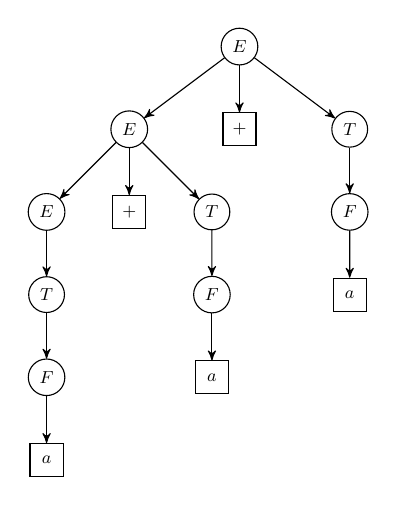
\begin{tikzpicture}[
  scale=0.7,
  transform shape,
  level 1/.style={sibling distance=2cm},
  level 2/.style={sibling distance=1.5cm},
  level 3/.style={sibling distance=1cm},
  level 4/.style={sibling distance=0.7cm},
  every node/.style={circle, draw, minimum size=0.6cm, font=\small}
]
  \node {$E$}
    child {node {$E$}
      child {node {$E$}
        child {node {$T$}
          child {node {$F$}
            child {node[rectangle] {$a$}}
          }
        }
      }
      child {node[rectangle] {$+$}}
      child {node {$T$}
        child {node {$F$}
          child {node[rectangle] {$a$}}
        }
      }
    }
    child {node[rectangle] {$+$}}
    child {node {$T$}
      child {node {$F$}
        child {node[rectangle] {$a$}}
      }
    };
\end{tikzpicture}
\end{center}
\end{minipage}

\subsection*{d. $((a))$}

\begin{center}
  \underline{Solution:}
\end{center}

\noindent
\begin{minipage}[t]{0.45\textwidth}
\textbf{Derivation:}

We derive the string $((a))$ from the start symbol $E$ as follows:

\begin{align*}
  E &\Rightarrow T \\
  &\Rightarrow F \\
  &\Rightarrow (E) \\
  &\Rightarrow (T) \\
  &\Rightarrow (F) \\
  &\Rightarrow ((E)) \\
  &\Rightarrow ((T)) \\
  &\Rightarrow ((F)) \\
  &\Rightarrow ((a))
\end{align*}
\end{minipage}
\hspace{0.5cm}
\vrule
\hspace{0.5cm}
\begin{minipage}[t]{0.5\textwidth}
\textbf{Parse Tree:}

\begin{center}
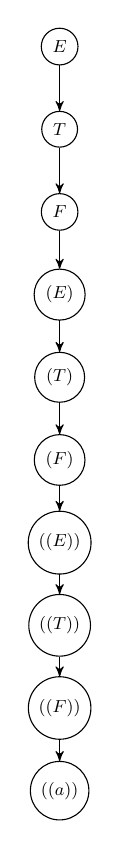
\begin{tikzpicture}[
  scale=0.7,
  transform shape,
  level 1/.style={sibling distance=2cm},
  level 2/.style={sibling distance=1.5cm},
  level 3/.style={sibling distance=1cm},
  level 4/.style={sibling distance=0.7cm},
  every node/.style={circle, draw, minimum size=0.6cm, font=\small}
]
  \node {$E$}
    child {node {$T$}
      child {node {$F$}
        child {node {$(E)$}
          child {node {$(T)$}
            child {node {$(F)$}
              child {node {$((E))$}
                child {node {$((T))$}
                  child {node {$((F))$}
                    child {node {$((a))$}
                    }
                  }
                }
              }
            }
          }
        }
      }
    };
\end{tikzpicture}
\end{center}
\end{minipage}
\newpage

\section*{2.4}
Give context-free grammars that generate the following languages. In all parts, the alphabet $\Sigma$ is $\{0,1\}$.

\subsection*{c. $\{w| \text{ the length of w is odd}\}$}

\begin{center}
  \underline{Solution:}
\end{center}

\begin{align*}
  S &\rightarrow ASA \: | \: A \\
  A &\rightarrow 0\:|\:1
\end{align*}

\subsection*{f. The empty set}
\begin{center}
  \underline{Solution:}
\end{center}
\begin{align*}
  S &\rightarrow S
\end{align*}

This language has a single rule that infinitely recurses and never terminates to any terminal symbols. Therefore, no words belong to this language.
\newpage

\section*{2.5}
Give informal descriptions and state diagrams of pushdown automata for the languages in Exercise 2.4.

\subsection*{c. $\{w| \text{ the length of w is odd}\}$}
\begin{align*}
  S &\rightarrow ASA \: | \: A \\
  A &\rightarrow 0\:|\:1
\end{align*}

\begin{center}
  \underline{Solution:}
\end{center}

\textbf{Informal Description:}

- The PDA starts in state $q_{start}$.

- It then pushes the symbols $\$S$ onto the stack and moves to state $q_{loop}$.

- On $q_{loop}$, it contains self transitions for all: 1. derivation rules, and 2. terminals.

- When all stack symbols have been consumed and only $\$$ remains, $q_{loop}$ transitions to $q_{accept}$.

- The PDA accepts the input string if both: 1. all symbols in the input string have been consumed, 2. the PDA is in the $q_{accept}$ state.

\vspace{0.5cm}

\textbf{State Diagram:}

\begin{center}
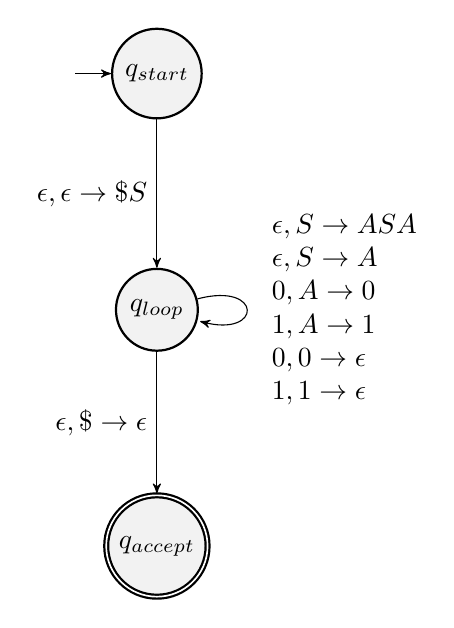
\begin{tikzpicture}[node distance=3cm, auto]
  % States
  \node[state, initial] (qi) {$q_{start}$};
  \node[state, below of=qi] (ql) {$q_{loop}$};
  \node[state, accepting, below of=ql] (qa) {$q_{accept}$};

  % Transitions
  \path[->]
    (qi) edge node[left] {$\epsilon, \epsilon \rightarrow \$S$} (ql)
    (ql) edge[loop right] node[right, align=left] {
    \: $\epsilon, S \rightarrow ASA$ \\
    \: $\epsilon, S \rightarrow A$ \\
    \: $0, A \rightarrow 0$ \\
    \: $1, A \rightarrow 1$ \\
    \: $0, 0 \rightarrow \epsilon$ \\
    \: $1, 1 \rightarrow \epsilon$
    } (ql)
    (ql) edge node[left] {$\epsilon, \$ \rightarrow \epsilon$} (qa);
\end{tikzpicture}
\end{center}


\subsection*{f. The empty set}
\begin{align*}
  S &\rightarrow S
\end{align*}

\begin{center}
  \underline{Solution:}
\end{center}

\textbf{Informal Description:}

- The PDA starts in state $q_{start}$.

- It then pushes the symbols $\$S$ onto the stack and moves to state $q_{loop}$.

- On $q_{loop}$, it contains an infinitely recursing self-transition that pops S and pushes it back again: $\epsilon, S \rightarrow S$.

- Thus, the symbol S is never consumed from the stack, and therefore the PDA never transitions to $q_{accept}$.

\vspace{0.5cm}

\textbf{State Diagram:}

\begin{center}
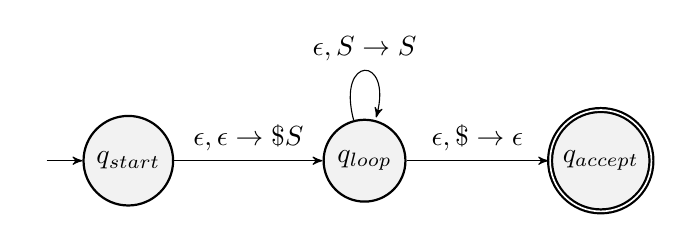
\begin{tikzpicture}[node distance=3cm, auto]
  % States
  \node[state, initial] (qi) {$q_{start}$};
  \node[state, right of=qi] (ql) {$q_{loop}$};
  \node[state, accepting, right of=ql] (qa) {$q_{accept}$};

  % Transitions
  \path[->]
    (qi) edge node[above] {$\epsilon, \epsilon \rightarrow \$S$} (ql)
    (ql) edge[loop above] node[above, align=left] {$\epsilon, S \rightarrow S$} (ql)
    (ql) edge node[above] {$\epsilon, \$ \rightarrow \epsilon$} (qa);
\end{tikzpicture}
\end{center}

\newpage

\section*{2.11}
Convert the CFG G4 given in Exercise 2.1 to an equivalent PDA, using the procedure given in Theorem 2.20.

\begin{align*}
  \left<EXPR\right> &\rightarrow \left<EXPR\right> + \left<TERM\right> \: | \: \left<TERM\right> \\
  \left<TERM\right> &\rightarrow \left<TERM\right> \times \left<FACTOR\right> \: | \: \left<FACTOR\right> \\
  \left<FACTOR\right> &\rightarrow \left(\left<EXPR\right>\right) \: | \: a
\end{align*}

\begin{center}
  \underline{Solution:}
\end{center}

\textbf{State Diagram:}

\begin{center}
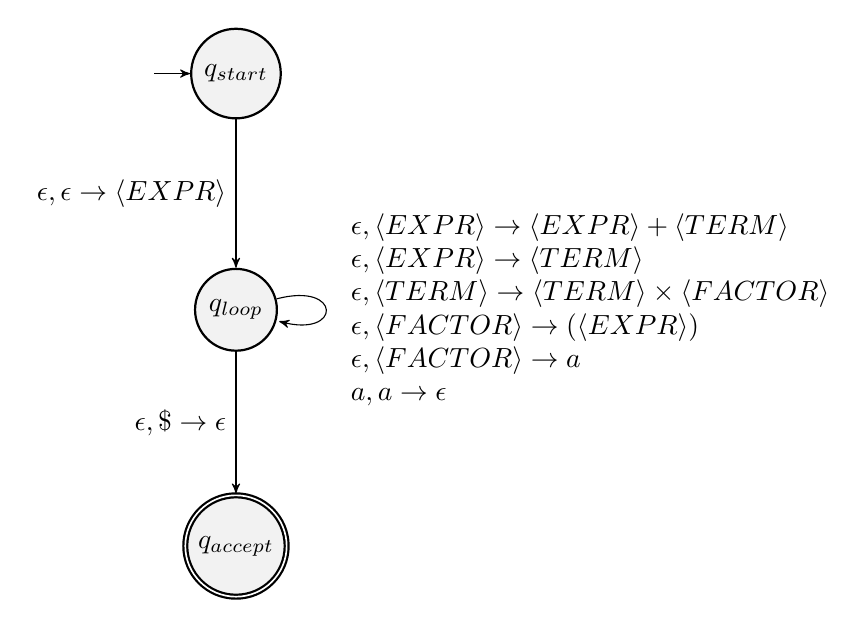
\begin{tikzpicture}[node distance=3cm, auto]
  % States
  \node[state, initial] (qi) {$q_{start}$};
  \node[state, below of=qi] (ql) {$q_{loop}$};
  \node[state, accepting, below of=ql] (qa) {$q_{accept}$};

  % Transitions
  \path[->]
    (qi) edge node[left] {$\epsilon, \epsilon \rightarrow \left<EXPR\right>$} (ql)

    (ql) edge[loop right] node[right, align=left] {
    \: $\epsilon, \left<EXPR\right> \rightarrow \left<EXPR\right> + \left<TERM\right>$ \\
    \: $\epsilon, \left<EXPR\right> \rightarrow \left<TERM\right>$ \\
    \: $\epsilon, \left<TERM\right> \rightarrow \left<TERM\right> \times \left<FACTOR\right>$ \\
    \: $\epsilon, \left<FACTOR\right> \rightarrow \left(\left<EXPR\right>\right)$ \\
    \: $\epsilon, \left<FACTOR\right> \rightarrow a$ \\
    \: $a, a \rightarrow \epsilon$
    } (ql)

    (ql) edge node[left] {$\epsilon, \$ \rightarrow \epsilon$} (qa);
\end{tikzpicture}
\end{center}

\newpage

\section*{2.13}

Let $G = (V, \Sigma, R, S)$ be the following grammar. $V = \{S, T, U\}$; $\Sigma = \{0, \#\}$; and
$R$ is the set of rules:

\begin{align*}
  S &\rightarrow TT | U \\
  T &\rightarrow 0T | T0 | \# \\
  U &\rightarrow 0U00 | \#
\end{align*}

a. Describe $L(G)$ in English.

b. Prove that $L(G)$ is not regular.

\begin{center}
  \underline{Solution:}
\end{center}

\subsection*{a.}
It's much simpler to describe $L(G)$ mathematically:

$L(G) = L(H) \cup L(K)$, where: 

$L(H) = \{w | w = 0^i \# o^{2i} \, \: \forall i \geq 1 \}$

$L(K) = \{w | w = 0^i \# 0^j \# 0^k, \: \forall i,k \geq 1, j \geq 0 \}$

\subsection*{b.}
\begin{proof}
  $ $

  Since regular languages are closed under the union operation and $L(G)$ is the union of 2 languages, then it is sufficient to show that any one of them is not regular.
  \newline
  
  We will show that $L(H)$ is not regular. We use the pumping lemma (for regular languages) to give a proof by contradiction.
  \newline

  Suppose for the sake of contradiction that $L(H)$ is regular. Since $L(H)$ is infinite, then there exists a pumping length $p$.
  \newline

  Take the string $w = 0^{p} \# 0^{2p} \in L(H)$.
  
  Since $|w| = 3p+1 \geq p$, then $w$ can be split as: $w = xyz$, where $|y| > 0$ and $|xy \leq p$.

  $\implies y = 0^k, \: 0 < k \leq p$

  $\implies w = 0^{p-k} 0^k \# 0^{2p}$

  $\implies xy^0z \in L(H)$

  $\implies 0^{p-k} \# 0^{2p} \in L(H)$

  $\implies 2(p-k) = 2p$

  $\implies k = 0$

  A contradiction.
  \newline

  Therefore, $L(H)$ is not regular.


  

  

  
\end{proof}

\newpage

\section*{2.14}
Convert the following CFG into an equivalent CFG in Chomsky normal form,
using the procedure given in Theorem 2.9.
\begin{align*}
  A &\rightarrow BAB \: | \: B \: | \: \epsilon \\
  B &\rightarrow 00 \: | \: \epsilon
\end{align*}

\begin{center}
  \underline{Solution:}
\end{center}

\textbf{\underline{Step 1: Add a new start variable $S_0$:}}

\begin{align*}
  S_0 &\rightarrow A \\
  A &\rightarrow BAB \: | \: B \: | \: \epsilon \\
  B &\rightarrow 00 \: | \: \epsilon
\end{align*}

\textbf{\underline{Step 2: Eliminate $\epsilon$ rules:}}
\newline

\underline{Step 2.1: Eliminate $B \rightarrow \epsilon$:}
\begin{align*}
  S_0 &\rightarrow A \\
  A &\rightarrow BAB \: | \: B \: | \: \epsilon \: | \: BA \: | AB \: A \\
  B &\rightarrow 00
\end{align*}
\newline

\underline{Step 2.2: Eliminate $A \rightarrow \epsilon$:}
\begin{align*}
  S_0 &\rightarrow A \: | \: \epsilon \\
  A &\rightarrow BAB \: | \: B \: | \: BA \: | AB \: A \\
  B &\rightarrow 00
\end{align*}


\textbf{\underline{Step 3: Eliminate unit rules:}}
\newline

\underline{Step 3.1: Eliminate $A \rightarrow A$:}
\begin{align*}
  S_0 &\rightarrow A \: | \: \epsilon \\
  A &\rightarrow BAB \: | \: B \: | \: BA \: | AB \\
  B &\rightarrow 00
\end{align*}

\underline{Step 3.2: Eliminate $S_0 \rightarrow A$:}
\begin{align*}
  S_0 &\rightarrow BAB \: | \: B \: | \: BA \: | AB \: | \: \epsilon \\
  A &\rightarrow BAB \: | \: B \: | \: BA \: | AB \\
  B &\rightarrow 00
\end{align*}

\underline{Step 3.3: Eliminate $A \rightarrow B$ and $S_0 \rightarrow B$:}
\begin{align*}
  S_0 &\rightarrow BAB \: | \: 00 \: | \: BA \: | AB \: | \: \epsilon \\
  A &\rightarrow BAB \: | \: 00 \: | \: BA \: | AB \\
  B &\rightarrow 00
\end{align*}

\textbf{\underline{Step 4: Introduce new variables to put the rules into proper Chomsky Normal Form form}}
\newline
\begin{align*}
  S_0 &\rightarrow BA_1 \: | \: 00 \: | \: BA \: | AB \: | \: \epsilon \\
  A &\rightarrow BA_1 \: | \: 00 \: | \: BA \: | AB \\
  A_1 &\rightarrow AB \\
  B &\rightarrow 00
\end{align*}

\newpage

\section*{2.23}
Let $D = \{xy| \: x, y \in \{0,1\}^*$ and $|x| = |y|$ but $x \neq y\}$.

\noindent
Show that D is a context-free language.

\begin{center}
  \underline{Solution:}
\end{center}

\textbf{Proof Idea: } Observe that in the language $D$, the left and right halves (x and  y) differ at some position: either $x$ has a $0$ where $y$ has a $1$, or $x$ has a $1$ where $y$ has a $0$. Construct a grammar that is the union of these 2 cases.
\newline

\begin{proof}
  $ $

  We prove that $D$ is context-free by defining a CFG for $D$.
  \newline

  Define a CFG that recognizes the union of these 2 languages:
  
  \indent
  \quad 1. $S_{01}$: The language whose words contain a 0 on the left half mismathed with a 1 in the corresponding position on the right half.
  
  \indent
  \quad 2. $S_{10}$: The language whose words contain a 1 on the left half mismathed with a 0 in the corresponding position on the right half.
  \newline

  Define:
  \begin{align*}
    V &= \{S, S_{01}, S_{10}, M, C\} \\
    \Sigma &= \{0, 1\} \\
    R &= \left\{
      \begin{aligned}
      S &\rightarrow S_{01} \: | \: S_{10}, \\
      S_{01} &\rightarrow 0M1 \: | \: 0S_{01}0 \: | \: 0S_{01}1 \: | \: 1S_{01}0 \: | \: 1S_{01}1, \\
      S_{10} &\rightarrow 1M0 \: | \: 0S_{10}0 \: | \: 0S_{10}1 \: | \: 1S_{10}0 \: | \: 1S_{10}1, \\
      M &\rightarrow CC \: | \: \epsilon, \\
      C &\rightarrow 0 \: | \: 1
      \end{aligned}
    \right\}
  \end{align*}

  The grammar $G = (V, \Sigma, R, S)$ is a CFG that recognizes the language $D$, therefore $D$ is a context-free language.

\end{proof}

\newpage

\section*{2.24}
Let $E = \{a^ib^j| \: i \neq j$ and $2i \neq j\}$.

\noindent
Show that E is a context-free language.

\begin{center}
  \underline{Solution:}
\end{center}

\textbf{Proof Idea:} Show that $E$ is defined as the union of 2 context-free languages: $F$ and $H$. Therefore, $E$ must be a context-free language.
\newline

\begin{proof}
  $ $

  Define:
  \begin{align*}
    F &= \{a^ib^j| \: i \neq j\} \\
    H &= \{a^ib^j| \: i \neq 2j\}
  \end{align*}

  This implies:
  \begin{align*}
    E &= F \cap H \\
      &= \bar{F} \cup \bar{H} \qquad \text{(By DeMorgan's law)}
  \end{align*}

  Where:
  \begin{align*}
    \bar{F} &= \{a^ib^j| \: i = j\} \\
    \bar{H} &= \{a^ib^j| \: i = 2j\}
  \end{align*}

  But clearly $\bar{F}$ and $\bar{H}$ are both \underline{deterministic} context-free languages (DCFLs).
  \newline

  Using the property of closure under complementation for DCFL, we get that both $F$ and $H$ are DCFLs.
  \newline

  Finally, using the property of closure under union for context-free languages, we conclude that $E$ is a DFCL.

\end{proof}

\newpage

\section*{2.26}
Show that if G is a CFG in Chomsky normal form, then for any string $w \in L(G)$
of length n $n \geq 1$, exactly $2n-1$ steps are required for any derivation of w.

\begin{center}
  \underline{Solution:}
\end{center}

\begin{proof}{By Strong Induction}
  $ $

  \underline{Base Case ($n=1$)}: 

  In this case the string $w$ is a single terminal symbol.
  
  In Chomsky Normal Form, such words are derived directly from the start variable with no extra derivations needed.

  Thus, it takes a single derivation. This matches the formula $2(1) -1 = 1$.
  \newline

  \underline{Inductive Step}:

  % Let $w$ be such that $|w| = k$, where $k \geq 1$.

  By the strong induction hypotheis, assume that the formula holds for all strings in $L(G)$ of length $1 \leq n \leq k$.
  \newline

  Let $w \in L(G)$ where $|w| = k+1$.
  
  \noindent
  $\implies |w| \geq 2$

  \noindent
  $\implies$ The first derivation rule of $w$ has the form: $S \rightarrow AB$, where $S$ is the start variable; $A$, $B$ are non-start variables. 
  Additionally, $w= p s$, where $A \Rightarrow^* p$ and $B \Rightarrow^* s$ and $p,s \neq \epsilon$ 
  \newline

  \noindent
  $\implies$
  \begin{align*}
    DerivationSteps(w) &= 1 + DerivationSteps(p) + DerivationSteps(s) \\
    &= 1 + DerivationSteps(p) + DerivationSteps(k+1-p) \\
    &= 1 + \left[2p - 1\right] + \left[2 \left(k+1-p\right) - 1 \right] \\
    &= 1 + \left[2p - 1\right] + \left[2 \left(k+1-p\right) - 1 \right] \\
    &= 1 + 2k \\
    &= 2(k+1) - 1. \\
  \end{align*}
  Therefore, the formula holds for $k+1$.
  
\end{proof}
\newpage

\section*{2.27}

Let $G = (V, \Sigma ,R, \left<STMT\right>)$ be the following grammar.
\begin{align*}
  \left<STMT\right> &\rightarrow \left<ASSIGN\right> | \left<IF-THEN\right> | \left<IF-THEN-ELSE\right> \\
  \left<IF-THEN\right> &\rightarrow \text{if condition then} \left<STMT\right> \\
  \left<IF-THEN-ELSE\right> &\rightarrow \text{if condition then} \left<STMT\right> \text{else} \left<STMT\right> \\
  \left<ASSIGN\right> &\rightarrow a:=1
\end{align*}

$\Sigma = \{if, \: condition, \: then, \: else, \: a:=1\}$

$V = \{<STMT>, \: <IF-THEN>, \: <IF-ELSE-THEN>, \: <ASSIGN>\}$
\newline

\noindent
G is a natural-looking grammar for a fragment of a programming language, but G
is ambiguous.
\newline

a. Show that G is ambiguous.

b. Give a new unambiguous grammar for the same language.

\subsection*{a.}

\begin{center}
  \underline{Solution:}
\end{center}

We prove this by showing a counter example.

The following word in $G$ has 2 different parse trees:
\begin{align*}
  w = \text{if condition then if condition then a:=1 else a:=1}
\end{align*}

In one parse tree the else belongs the outer if, and in another parse tree it belongs to the inner if.
Therefore, this grammar is ambiguous.

This problem is called: the dangling else ambiguity.

\subsection*{b.}

\begin{center}
  \underline{Solution:}
\end{center}

\begin{align*}
  \left<STMT\right> &\rightarrow \left<MATCHED\right> \: | \: \left<UNMATCHED\right> \\
  \left<MATCHED\right> &\rightarrow \left<ASSIGN\right> \: | \: \text{if condition then } \left<MATCHED\right> \text{ else } \left<MATCHED\right> \\ 
  \left<UNMATCHED\right> &\rightarrow \text{if condition then } \left<STMT\right> \: | \: \text{if condition then } \left<MATCHED\right> else \left<UNMATCHED\right> \\
  \left<ASSIGN\right> &\rightarrow a:=1
\end{align*}



\newpage

\section*{2.30}
Use the pumping lemma to show that the following languages are not context free.

\subsection*{d.}
\begin{align*}
  L = \Bigl\{t1\#t2\# \ldots \#t_k| \: k \geq 2, \forall i \: t_i \in \{a, b\}^* \: \land \: \exists i,j: (t_i = t_j \: \land \: i \neq j)\Bigr\}
\end{align*}

\begin{center}
  \underline{Solution:}
\end{center}

\begin{proof}
  We use the pumping lemma for context-free languages to show that $L$ is not context-free.
  \newline

  Assume for the sake of contradiction that $L$ is a CFL. Let $p$ be the pumping length given by the pumping lemma.
  \newline

  Consider the string $s = a^p b^p \# a^p b^p$.
  \newline

  Clearly, $s \in L$ because it has $k=2$ parts, and $t_1 = a^p b^p = t_2$.
  \newline

  We show that for any decomposition $s = uvxyz$ satisfying $|vxy| \le p$ and $|vy| > 0$, there exists an $i \ge 0$ such that $uv^ixy^iz \notin L$.
  \newline

  \textbf{Case 1:} The substring $vxy$ does not contain the symbol $\#$.
  
  In this case, $vxy$ must be entirely contained within either the first part ($t_1$) or the second part ($t_2$). This is because $|vxy| \le p$, so it cannot span across the $\#$ without containing it.
  
  Without loss of generality, assume $vxy$ is in the first part.
  Pump up with $i=2$. The resulting string is $s' = t_1' \# t_2$.
  Since $|vy| > 0$, we have $|t_1'| \neq |t_1|$.
  Since $|t_1| = |t_2|$, it follows that $|t_1'| \neq |t_2|$, and thus $t_1' \neq t_2$.
  Since there are only 2 parts ($k=2$), and they are not equal, the condition $\exists i,j: (t_i = t_j \land i \neq j)$ is not satisfied.
  Thus $s' \notin L$.
  \newline

  \textbf{Case 2:} The substring $vxy$ contains the symbol $\#$.
  
  Since $|vxy| \le p$, $vxy$ must be a substring of the segment $b^p \# a^p$ (the $b$'s from $t_1$ and $a$'s from $t_2$).
  
  \textbf{Subcase 2a:} The symbol $\#$ is in $x$.
  Then $v$ consists of $b$'s from $t_1$, and $y$ consists of $a$'s from $t_2$.
  Let $v = b^m$ and $y = a^n$, with $m+n > 0$.
  Pump up with $i=2$. The resulting string is $s' = a^p b^{p+m} \# a^{p+n} b^p$.
  For $s'$ to be in $L$, we must have $t_1' = t_2'$, i.e., $a^p b^{p+m} = a^{p+n} b^p$.
  Comparing the number of $a$'s, we need $p = p+n \implies n=0$.
  Comparing the number of $b$'s, we need $p+m = p \implies m=0$.
  This contradicts $|vy| > 0$.
  Thus $t_1' \neq t_2'$, so $s' \notin L$.
  \newline

  \textbf{Subcase 2b:} The symbol $\#$ is in $v$ or $y$.
  Pump down with $i=0$. This removes the $\#$ from the string.
  The resulting string has no $\#$ symbol, meaning it consists of a single part ($k=1$).
  However, the definition of $L$ requires $k \ge 2$.
  Thus the pumped string is not in $L$.
  \newline

  In all cases, we found a pumped string that is not in $L$. This contradicts the pumping lemma.
  Therefore, $L$ is not context-free.
  
\end{proof}
\newpage

\section*{2.31}
Let B be the language of all palindromes over $\{0,1\}$ containing equal numbers of
0s and 1s. Show that B is not context free.

\begin{center}
  \underline{Solution:}
\end{center}

\begin{proof}
  We use the pumping lemma for context-free languages to show that $B$ is not context-free.
  
  Assume for the sake of contradiction that $B$ is a CFL. Let $p$ be the pumping length given by the pumping lemma.
  
  Consider the string $s = 0^p 1^{2p} 0^p$.
  
  First, we verify that $s \in B$:
  \begin{itemize}
    \item $s$ reads the same forwards and backwards, so it is a palindrome.
    \item The number of 0s is $p + p = 2p$. The number of 1s is $2p$. Thus, it has equal numbers of 0s and 1s.
  \end{itemize}
  Also, $|s| = 4p \ge p$.
  
  We show that for any decomposition $s = uvxyz$ satisfying $|vxy| \le p$ and $|vy| > 0$, the pumped string is not in $B$.
  
  Since $|vxy| \le p$, the substring $vxy$ cannot span across the block of 1s to touch both blocks of 0s (the distance between the two blocks of 0s is $2p > p$).
  
  We consider the cases for the position of $vxy$:
  \newline

  \textbf{Case 1:} $vxy$ is contained in the first $0^p$ or overlaps the first $0^p$ and $1^{2p}$.
  
  Pump up with $i=2$ ($uv^2xy^2z$). This increases the number of 0s in the first block (or 0s in first block and 1s in middle), but the last block of 0s remains $0^p$. The resulting string is not a palindrome because it starts with more 0s than it ends with (or has mismatched structure). Hence, it is not in $B$.
  \newline

  \textbf{Case 2:} $vxy$ is contained entirely within $1^{2p}$.
  
  Pump up with $i=2$. This increases the number of 1s, but the number of 0s remains $2p$. The number of 1s becomes $2p + |vy| > 2p$. The condition that the number of 0s equals the number of 1s is violated. Hence, it is not in $B$.
  \newline

  \textbf{Case 3:} $vxy$ overlaps $1^{2p}$ and the last $0^p$, or is contained in the last $0^p$.
  
  Pump up with $i=2$. This increases the number of 0s in the last block, but the first block remains $0^p$. The resulting string is not a palindrome. Hence, it is not in $B$.
  \newline
  
  In all cases, the pumped string is not in $B$. This contradicts the pumping lemma.
  Therefore, $B$ is not context-free.

\end{proof}


\end{document}